\documentclass{article}

\usepackage{graphicx}
\DeclareGraphicsExtensions{.pdf,.png,.jpg,.jpeg}

\begin{document}

\setcounter{page}{10}

\section*{Observational Data}
{
The value of the Motor Constant $K_m$ was found by changing the attached weight's mass, and then finding the highest speed at which the car wouldn't move. The following graph is the linearized plot of the recorded data:
\\
\\
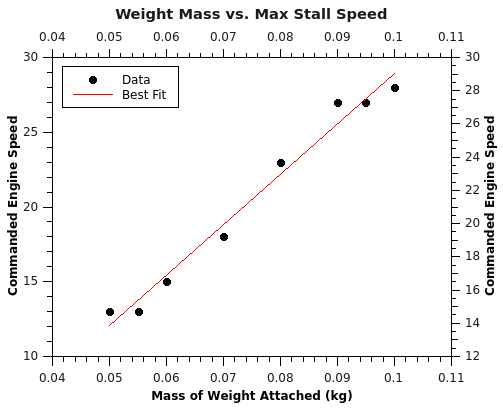
\includegraphics[width=14cm]{MotorConstantGraph.png}
\\
\\
From the graph and the relationship with the motor constant, we can calculate it to be:
\\
\\
\[ K_m = \frac{\Delta M g}{\Delta C_u} = 0.0291 \]

\pagebreak

In order to find the value of the coefficient of friction, $b$, we can compare the simulated system to that of the actual car for different values of $b$. The following graph showcases the effect that different values have on the system along with the recorded observed system response:
\\
\\
\center{
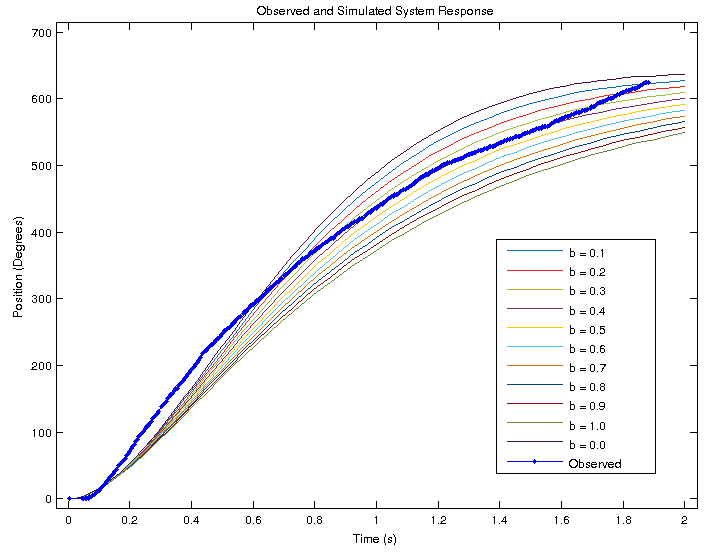
\includegraphics[width=14cm]{ComparitiveAnalysis.png}
}
}
\\
\\
If we compare the actual response to that of the simulation, we see that the closest value of $b$ which approximates the system is:
\\
\[ b = 0.4 \]
\\
\pagebreak
\\
If we isolate the simulation with our chosen value of $b$ and plot it against our output we get:
\\
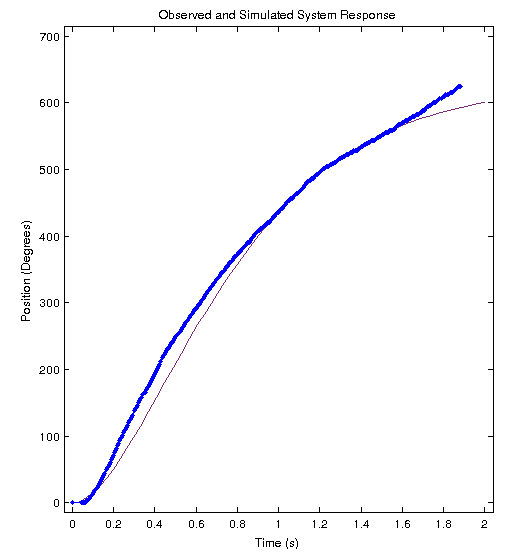
\includegraphics[width=14cm]{ChosenSimComparitive.png}
\end{document}